\section{GenLayers} \label{sec:GenLayers}

This utility generates two monolayers composed of molecules specified in a
\texttt{FIELD}-like file. For now, only one type of molecule is used (the
first one in the \texttt{FIELD}-like file; other molecule types are
ignored). The two layers are mirror images of each other, that is,
molecules in both layers are grown from box edge to box middle. The layers
are placed in $z$ direction (that is, on $xy$ planes of the simulation
box).

The first beads of the molecules are arranged on a square lattice defined
either by given spacing in $x$ and $y$ directions (\texttt{-s} option) or
by the number of molecules per layer (\texttt{-nm} option). The rest of the
beads of each molecule are placed based on the coordinates in the
\texttt{FIELD}-like file. By default, \texttt{GenLayers} places the two
mirror layers at the edges of a simulation box; using \texttt{-g}
option, a gap from box edge can be introduced. Therefore, this utility
can generate, for example, polymer brushes at box edges or a double layer
(such as a biological membrane) in the middle of the box.

By default, the total number of beads in the generated system is equal to
three times the box volume, that is, the typical number of beads in
dissipative particle dynamics simulations. Beads that are not in the
molecules, are put at the beginning of the output files (i.e., they have
lower indices) with coordinates of the box centre, and name \texttt{None}.
The idea is that once the layers are generated, \texttt{AddToSystem}
utility (Section~\ref{sec:AddToSystem}) can be used to exchange these
excess beads for different species. The \texttt{-n} option changes the
total number of beads. If the number is lower than the total number of
beads needed to construct the two layers of molecules, it is adjusted to
exactly that number.

The input \texttt{FIELD}-like file must contain \texttt{species} and
\texttt{molecule} sections (although, only the first molecule is considered
and \texttt{nummols} is disregarded), but the \texttt{interaction} section
is ignored (see \texttt{DL\_MESO} manual for details on the \texttt{FIELD}
file or below for a simple example). The first line of the
\texttt{FIELD}-like file, that is ignored by \texttt{DL\_MESO}, must start
with box dimensions, i.e., with three numbers.

This utility does not have error checking for the provided
\texttt{FIELD}-like file. If the file is not correct, \texttt{GenLayers}
will exhibit undefined behaviour, that is, it will either freeze, crash, or
run without errors, producing unexpected output files.

The following \texttt{vmd}-generated snapshot (the transparent squares are
just a visual aid) is an example output using command \texttt{GenLayers
out.vsf out.vcf -n 1 -nm 50 -g 1} and the provided \texttt{FIELD}-like
file:

\hfill
\begin{minipage}{0.4\textwidth}

  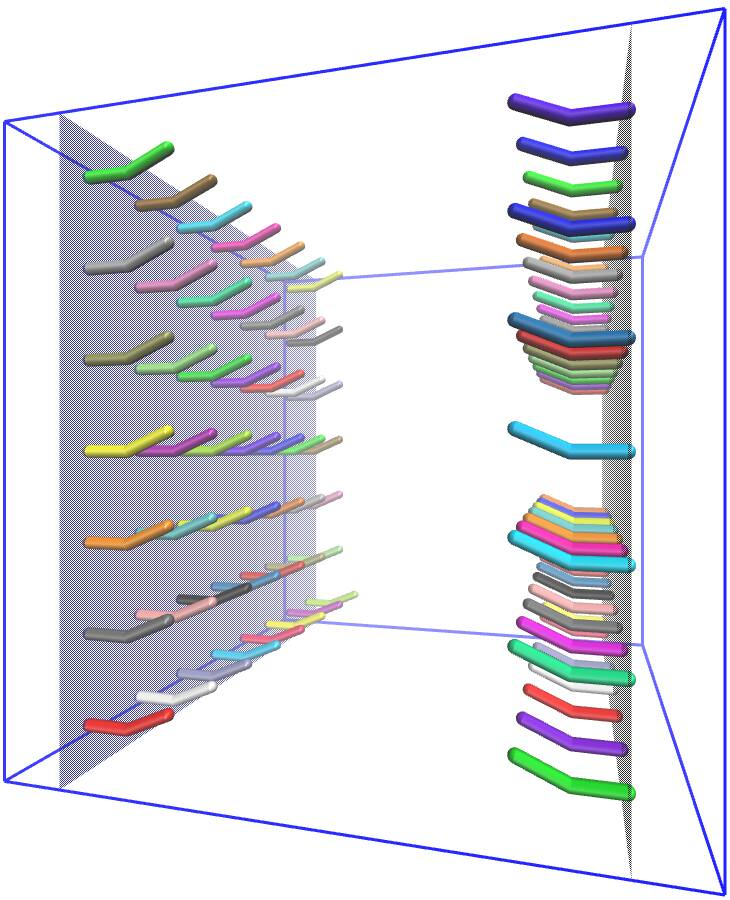
\includegraphics[width=\textwidth]{GenLayers-478ctac.jpg}
\end{minipage}
\hfill
\begin{minipage}{0.3\textwidth}
  \centering
  \texttt{FIELD}-like file
  \vspace{-1em}

\begin{verbatim}
   10 10 10
   species 1
   A   1.0 0.0 0
   molecules 1
   A3
   nummols 1
   beads 3
   A 0 0.0 0.0
   A 0 0.0 0.7
   A 0 0.3 1.4
   bonds 2
   harm 1 2 100.0 0.7
   harm 2 3 100.0 0.7
   finish
\end{verbatim}
\end{minipage}

The utility generates \texttt{vsf} structure and \texttt{vcf} coordinate
files.

Usage (\texttt{GenLayers} does not use standard options):

\vspace{1em}
\noindent
\texttt{GenLayers <out.vsf> <out.vcf> <options>}

\noindent
\begin{longtable}{p{0.15\textwidth}p{0.794\textwidth}}
  \toprule
  \multicolumn{2}{l}{Mandatory arguments} \\
  \midrule
  \texttt{<out.vsf>} & output \texttt{vsf} structure file \\
  \texttt{<out.vcf>} & output \texttt{vcf} coordinate file \\
  \toprule
  \multicolumn{2}{l}{Options} \\
  \midrule
  \texttt{-s <x> <y>} & spacing of molecules in $x$ and $y$ directions
    (default: 1 1) \\
  \texttt{-n <int>} & total number of beads (default: three times the box
    volume)\\
  \texttt{-nm <int>} & number of molecules in each layer (rewrites
    \texttt{-s} option) \\
  \texttt{-g <float>} & gap between box edges and the molecules (default: 0)\\
  \texttt{-f <name>} & \texttt{FIELD}-like file (default: \texttt{FIELD}) \\
  \texttt{-v}        & verbose output that provides information about all
    bead and molecule types \\
  \texttt{-h}        & print this help and exit \\
  \bottomrule
\end{longtable}
